% \chapter{Fractures}
% \chapter{Introduction}
\begin{figure}[htpb]%
    \centering%
    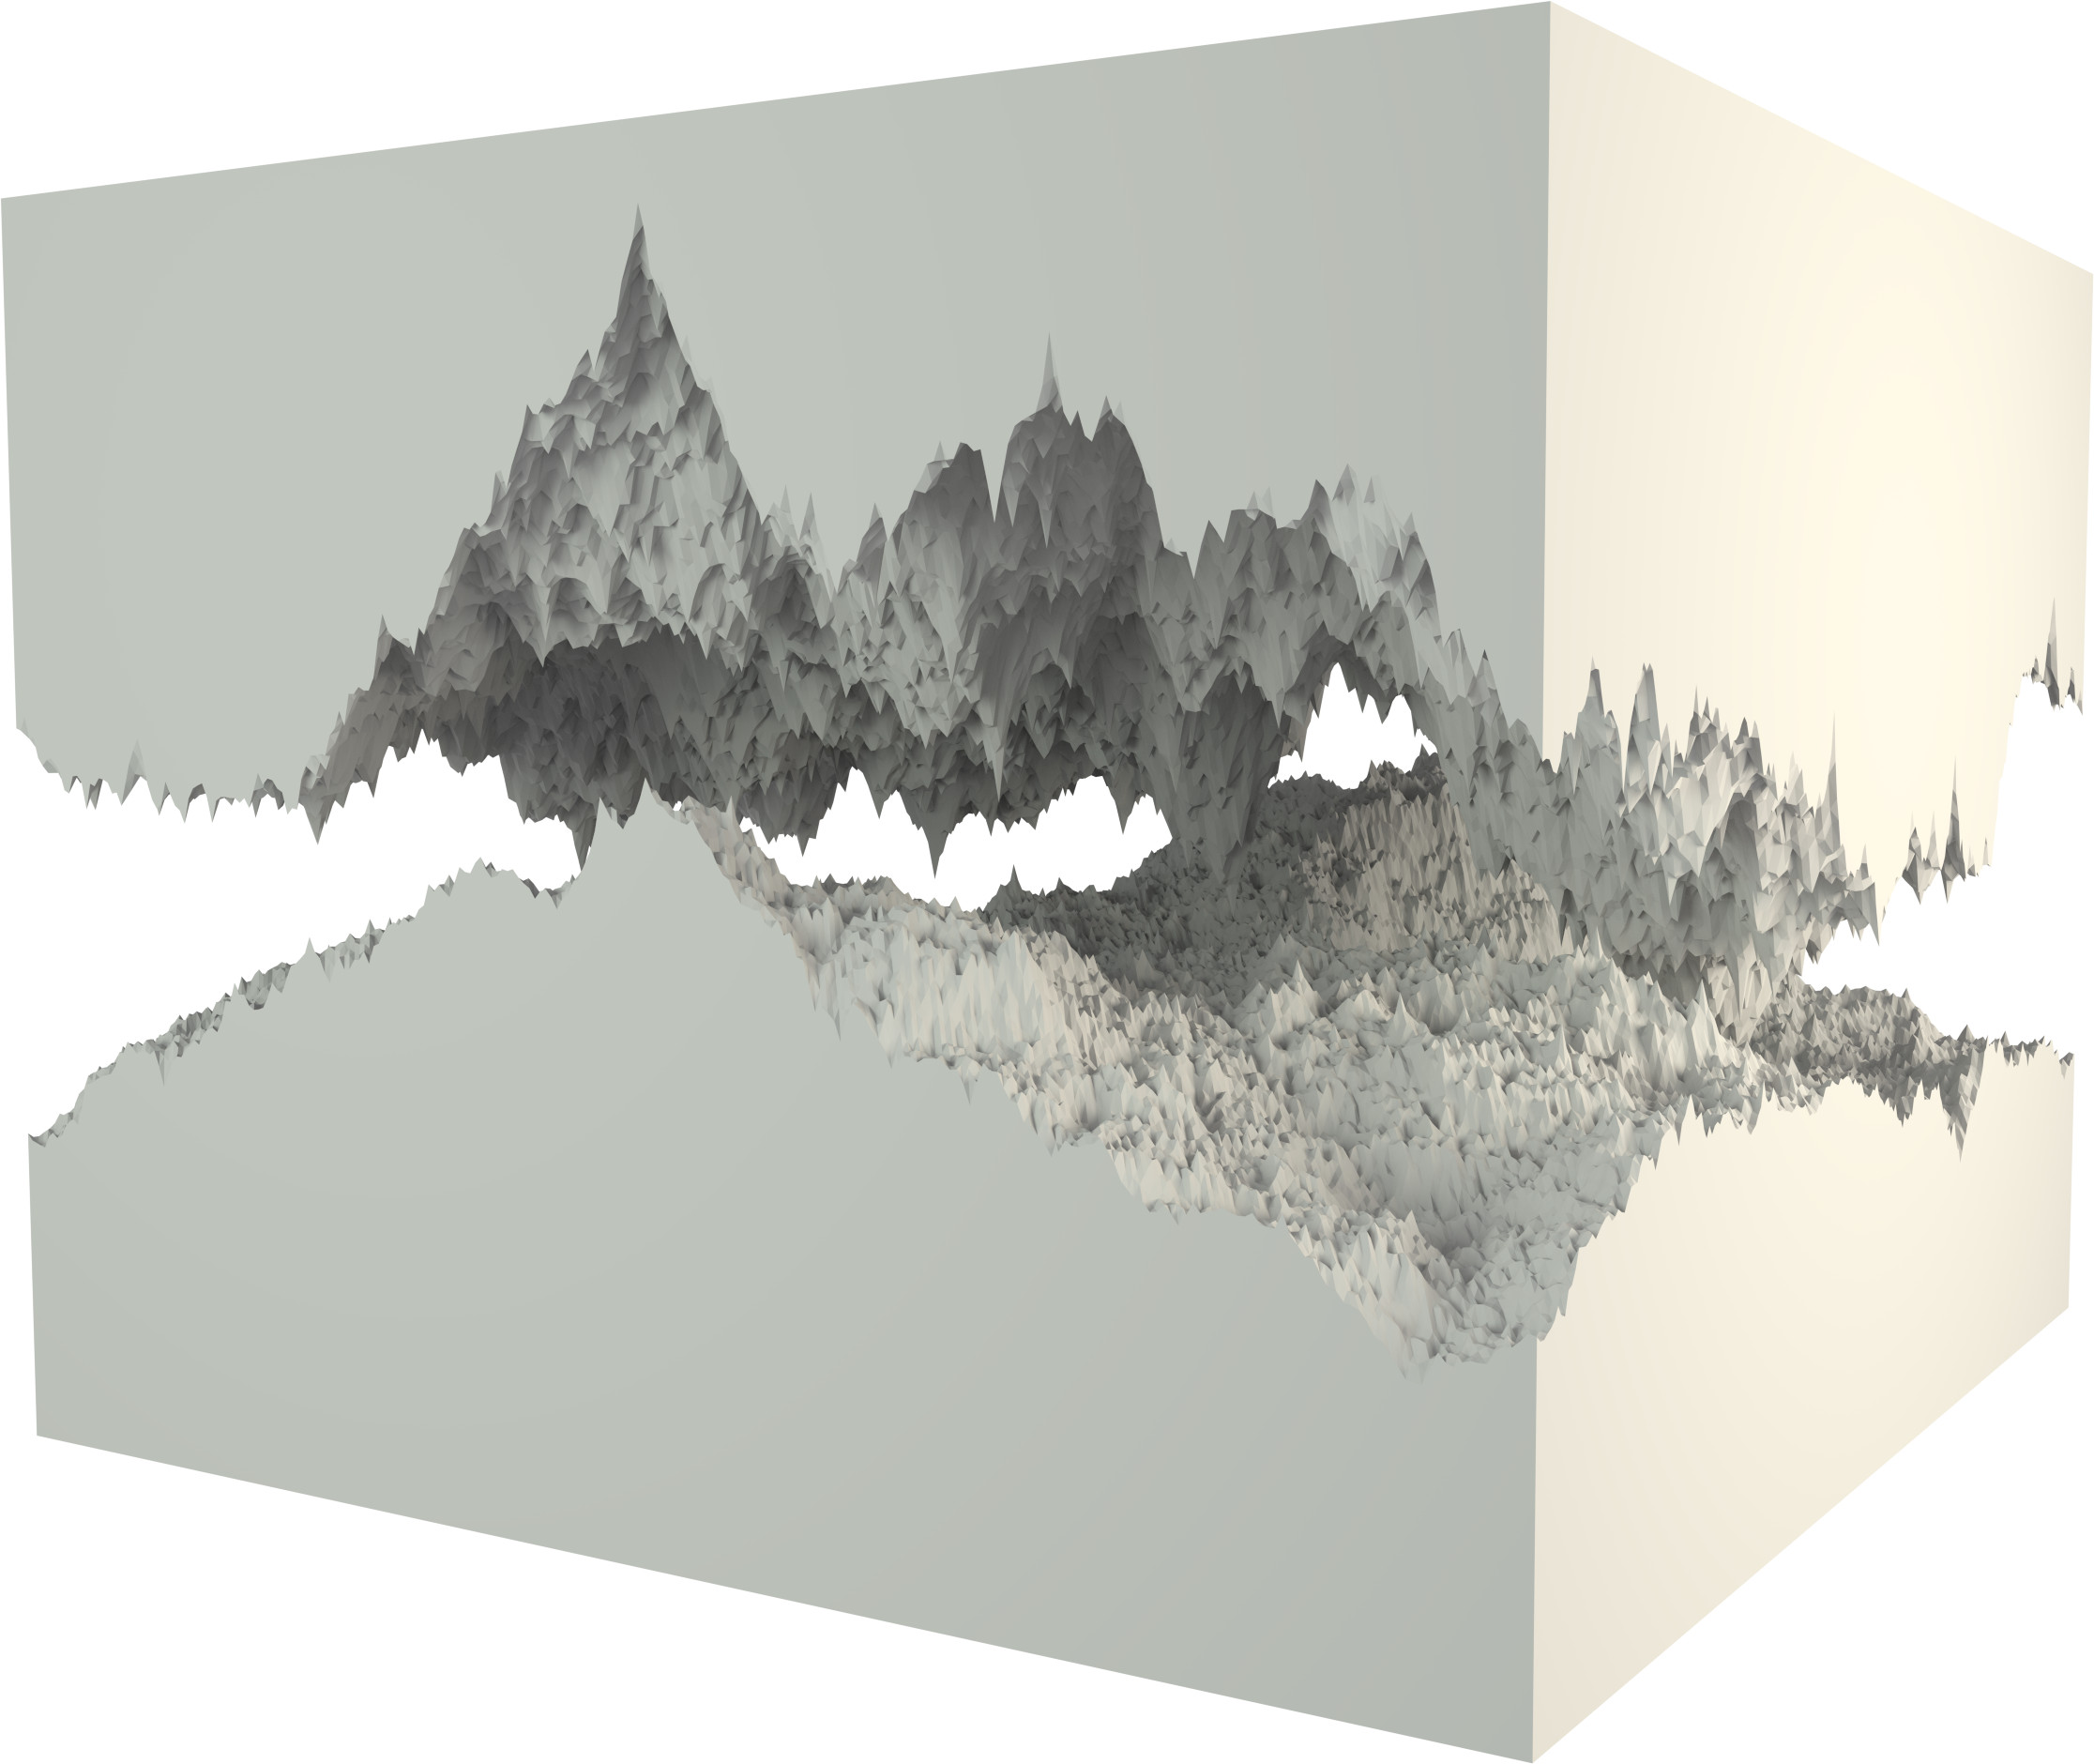
\includegraphics[width=\textwidth]{images/fracture/large_fracture05.jpg}%
    \caption{Caption}%
\end{figure}%

\chapter{Introduction}
We want to study the behaviour of water trapped in nanoscale (pores and) fractures in silica, so need want a way to generate and characterize such a structure. (Several methods of characterizing a fracture could be imagined (\hl{SOURCES, examples}), and we will use several of them.)        

\hl{terrain == heightmap??, finn bra ord her}

\orangebox{
    \begin{itemize}
        \item Plot 1D DMA estimate vs. synthesized 1D fBm from FracLab. Difference between with and without new $f^*$.
        \item Plot 2D DMA estimate vs. synth. 2D fBm from FracLab? \hl{Does FracLab generated 2D?}
        \item Plot 2D DMA est. vs. input Hurst for diamond square. Compare with and without addition and PBC.
    \end{itemize}

}

\chapter{Characterization}

\todo{change wording? copied from Fractals...}
An \emph{affine transformation} transforms a point $\bvec x = (x_1, \dots, x_n)$ into new points $\bvec x' = (r_1x_1, \dots, r_n, x_n)$, where the scaling rations $r_1, \dots, r_n$ are \emph{not} all equal.

A bounded set $\mathcal{S}$ is \emph{self-affine} if $\mathcal{S}$ is the union of $N$ non-overlapping subsets $\mathcal{S}_1, \dots, \mathcal{S}_N$, each of which is congruent to the set $\bvec r(\mathcal{S})$ obtained from $\mathcal S$ by the affine transform defined by $\bvec r$. Here \emph{congruent} means that the set of points $\mathcal{S}$ is identical to the set of points $\bvec r(\mathcal{S})$ after possible translations and/or rotations of the set\cite{feder1988fractals}.

A set $\mathcal{S}$ is \emph{statistically self-affine} if $\mathcal{S}$ is the union of $N$ non-overlapping subsets each of which is scaled down by $\bvec r$ from the original, and is identical in all statistical respects to $\bvec r(\mathcal{S})$.

% \section{Surface area}
% \section{Distance to nearest atom}
\begin{itemize}
    \item Fractals
    \item Fractional Brownian Motion
    \item The Hurst Exponent
\end{itemize}
